%!TEX program = xelatex
% =============================================================================
% PRESENTACIÓN — Evaluación 3 ECSD · Caso 2: Línea de Producción con Balanceo Dinámico
% Estilo: minimalista, tipografía DIN condensada, acento teal.
% Compilar con XeLaTeX. En Overleaf: subir el repo y elegir XeLaTeX en Menú →
% Compiler; las fuentes caen solas a Lato + Roboto Condensed.
% Las figuras se generan con informe/figuras/generar_figuras.py
% =============================================================================
\documentclass[aspectratio=169,10pt]{beamer}

\usepackage[spanish, es-tabla]{babel}
\deactivatequoting
\usepackage{graphicx}
\usepackage{booktabs}
\usepackage{array}
\usepackage{tikz}
\usetikzlibrary{shapes.geometric, arrows, positioning, calc}

\usepackage{fontspec}

% Tipografía en cascada: primero las de Windows (el diseño original), después
% las libres del árbol de TeX Live — que es lo que hay en Overleaf, donde las
% de Microsoft no existen —, y al final las genéricas para que la compilación
% nunca falle por fuentes.
\IfFontExistsTF{Segoe UI}
  {\setsansfont{Segoe UI}}
  {\IfFontExistsTF{Lato-Regular.ttf}
    {\setsansfont{Lato}[
       Extension = .ttf, UprightFont = *-Regular, BoldFont = *-Bold,
       ItalicFont = *-Italic, BoldItalicFont = *-BoldItalic]}
    {}}

% La condensada de los titulares y las cifras grandes: Roboto Condensed, del
% árbol de TeX Live.
%
% Antes era Bahnschrift, la condensada de Windows. Se cambió porque es una
% fuente variable en un solo archivo y dvipdfmx no sabe incrustarla: la lee
% como una colección TTC y aborta con «Invalid TTC index / Invalid font: -1».
% Compilaba en la máquina donde se generó el PDF versionado, pero no en la
% otra. Roboto Condensed es estática, da el mismo aire DIN, y sale igual acá
% y en Overleaf.
\IfFontExistsTF{RobotoCondensed-Regular.otf}
  {\newfontfamily\dinfont{RobotoCondensed}[
     Extension = .otf, UprightFont = *-Regular, BoldFont = *-Bold,
     ItalicFont = *-Italic]}
  {\newcommand{\dinfont}{\sffamily}}

% Las figuras (y el logo) se buscan igual desde presentacion/ o desde la raíz.
\graphicspath{{../informe/figuras/}{informe/figuras/}{../informe/}{informe/}{figuras/}{./}}

% ── Colores (estilo deck Seguridad + acentos del proyecto) ───────────────────
\definecolor{marino}{HTML}{1A2744}
\definecolor{grisazul}{HTML}{4A5568}
\definecolor{tealu}{HTML}{009B8A}
\definecolor{ambar}{HTML}{E8A013}
\definecolor{rojo}{HTML}{D03B3B}
\definecolor{grisclaro}{HTML}{EDECE7}

% ── Beamer minimalista ───────────────────────────────────────────────────────
\setbeamertemplate{navigation symbols}{}
\setbeamertemplate{itemize item}{\textcolor{tealu}{\raisebox{0.12ex}{\scriptsize$\blacksquare$}}}
\setbeamertemplate{itemize subitem}{\textcolor{grisazul}{--}}
\setbeamercolor{normal text}{fg=marino}
\setbeamercolor{itemize/enumerate body}{fg=marino}
\setbeamerfont{normal text}{size=\small}
\setbeamertemplate{frametitle}{}
\setbeamertemplate{footline}{%
  \hspace{1.2em}\raisebox{1.1em}{\tiny\color{grisazul}%
  ECSD · Evaluación 3 — Caso 2 · César Olivares · Simón García-Huidobro}%
  \hfill\raisebox{1.1em}{\tiny\color{grisazul}\insertframenumber\ /\ \inserttotalframenumber\hspace{1.2em}}}

% Título de lámina: título en mayúsculas + subtítulo gris.
% Antes llevaba delante un número de tema en gris claro. Se quitó: contaba
% temas, no páginas, así que a partir de la segunda lámina ya no coincidía con
% el número del pie y desorientaba en vez de orientar. El pie sigue llevando la
% numeración real de páginas.
\newcommand{\titulo}[2]{%
  \vspace{0.12cm}%
  {\dinfont\LARGE\color{marino}\MakeUppercase{#1}}\\[0.3ex]
  {\normalsize\color{grisazul}#2}\\[0.2ex]
  {\color{tealu}\rule{2.2cm}{2pt}}\\[0.6ex]}

% Tarjeta para conclusiones / bloques
\newcommand{\tarjeta}[2]{%
  \begin{beamercolorbox}[wd=\linewidth, sep=5pt, rounded=true]{tarjetabox}%
  {\small\bfseries\color{marino}#1}\\[2pt]{\footnotesize\color{grisazul}#2}%
  \end{beamercolorbox}}
\setbeamercolor{tarjetabox}{bg=grisclaro}

% Número gigante (indicador tipo "stat tile")
\newcommand{\cifra}[2]{%
  \begin{center}{\dinfont\fontsize{34}{36}\selectfont\color{tealu}#1}\\[2pt]
  {\footnotesize\color{grisazul}#2}\end{center}}

\newcolumntype{L}[1]{>{\raggedright\arraybackslash}p{#1}}

\tikzset{
  etapac/.style={rectangle, rounded corners, minimum width=2.05cm, minimum height=1.0cm,
                 text centered, draw=marino, fill=grisclaro, font=\scriptsize, align=center},
  etaparc/.style={rectangle, rounded corners, minimum width=2.05cm, minimum height=1.0cm,
                  text centered, draw=tealu, fill=tealu!15, font=\scriptsize\bfseries, align=center},
  etapachica/.style={rectangle, rounded corners, minimum width=1.55cm, minimum height=0.8cm,
                 text centered, draw=marino, fill=grisclaro, font=\tiny, align=center},
  etaparchica/.style={rectangle, rounded corners, minimum width=1.55cm, minimum height=0.65cm,
                  text centered, draw=tealu, fill=tealu!15, font=\tiny\bfseries, align=center},
  colaq/.style={rectangle, minimum width=0.95cm, minimum height=0.6cm, text centered,
                draw=grisazul!60, fill=ambar!12, font=\tiny},
  nodo/.style={rectangle, rounded corners, draw=tealu, fill=tealu!8, font=\scriptsize\bfseries, inner sep=7pt},
  arrow/.style={thick,->,>=stealth,color=marino},
  rep/.style={rectangle, rounded corners, draw=marino, fill=grisclaro, font=\scriptsize, minimum width=1.65cm, minimum height=0.55cm},
  colabox/.style={rectangle, draw=grisazul!60, fill=ambar!12, font=\scriptsize\bfseries, minimum width=1.9cm, minimum height=0.55cm},
  paso/.style={rectangle, rounded corners, draw=marino, fill=grisclaro, font=\tiny, align=center,
               minimum width=3.0cm, minimum height=0.62cm, inner sep=3pt},
  pasoc/.style={rectangle, rounded corners, draw=tealu, fill=tealu!12, font=\tiny\bfseries, align=center,
               minimum width=3.0cm, minimum height=0.62cm, inner sep=3pt},
  pasor/.style={rectangle, rounded corners, draw=rojo, fill=rojo!8, font=\tiny, align=center,
               minimum width=3.0cm, minimum height=0.62cm, inner sep=3pt}
}

\begin{document}

% ── 1 · PORTADA ──────────────────────────────────────────────────────────────
\begin{frame}[plain]
\vfill
\begin{center}

\includegraphics[height=1.7cm]{logoBN.png}\\[10pt]
{\dinfont\small\color{grisazul}UNIVERSIDAD DE SANTIAGO DE CHILE}\\[2pt]
{\dinfont\small\color{grisazul}ESTRUCTURA DE COMPUTADORES Y SISTEMAS DISTRIBUIDOS · EVALUACIÓN 3 · CASO 2}\\[14pt]
{\dinfont\fontsize{26}{31}\selectfont\color{marino}Línea de producción con\\balanceo dinámico de carga}\\[12pt]
{\normalsize\color{grisazul}Sistema distribuido que simula una planta conservera, detecta su cuello\\de botella en vivo y demuestra qué pasa cuando se escala la etapa lenta}\\[18pt]
{\small\color{marino}\textbf{César Olivares · Simón García-Huidobro}}\\[4pt]
{\small\color{grisazul}Profesor: Daniel Calderón R. · 26 de agosto de 2026}
\end{center}
\vfill
\end{frame}

% ── 2 · EL PROBLEMA (nivel general, antes del caso) ──────────────────────────
\begin{frame}
\titulo{El problema}{Toda línea en serie produce al ritmo de su etapa más lenta — y sin medición no se sabe cuál es}
\begin{center}
\resizebox{0.96\linewidth}{!}{%
\begin{tikzpicture}
  % Panel izquierdo: sin el desarrollo
  \node [font=\scriptsize\bfseries\color{marino}] at (0,2.15) {Sin el desarrollo};
  \node (a1) [etapachica] at (-2.4,1.2) {Etapa A\\ ciclo corto};
  \node (q1) [colaq, minimum width=1.35cm] at (-0.5,1.2) {\#6 \#5 \#4 \#3};
  \node (b1) [etapachica, draw=rojo, fill=rojo!8] at (1.3,1.2) {\textbf{Etapa B}\\ ciclo largo};
  \node (c1) [etapachica] at (3.2,1.2) {Etapa C\\ ciclo corto};
  \draw [arrow] (a1) -- (q1); \draw [arrow] (q1) -- (b1); \draw [arrow] (b1) -- (c1);
  \node [font=\tiny\color{rojo}, align=center] at (0.4,0.35) {el trabajo en curso se acumula frente\\ a la etapa lenta, sin límite y sin aviso};
  % Panel derecho: con el desarrollo
  \node [font=\scriptsize\bfseries\color{tealu}] at (11.6,2.6) {Con el desarrollo};
  \node (a2) [etapachica] at (7.0,1.2) {Etapa A};
  \node (q2) [colaq] at (8.6,1.2) {\#3};
  \node (b2a) [etaparchica] at (10.3,1.7) {B — réplica 1};
  \node (b2b) [etaparchica] at (10.3,0.7) {B — réplica 2};
  \node (c2) [etapachica] at (12.2,1.2) {Etapa C};
  \draw [arrow] (a2) -- (q2);
  \draw [arrow] (q2.east) -- (b2a.west); \draw [arrow] (q2.east) -- (b2b.west);
  \draw [arrow] (b2a.east) -- (c2.west); \draw [arrow] (b2b.east) -- (c2.west);
  \node (det) [rectangle, rounded corners, draw=tealu, dashed, font=\tiny\bfseries\color{tealu},
               align=center, inner sep=3pt] at (8.6,2.6) {detector: mide la fila\\ de cada etapa};
  \draw [thick, dashed, ->, >=stealth, color=tealu] (det.south) -- (q2.north);
  \node [font=\tiny\color{tealu}, align=center] at (9.6,0.0) {se mide dónde crece la fila y se agrega\\ capacidad exactamente en esa etapa};
\end{tikzpicture}}
\end{center}
\begin{itemize}
  \item Dos problemas de ingeniería: \textbf{(1)} repartir el trabajo entre copias de la etapa lenta sin duplicar ni perder unidades, y \textbf{(2)} determinar, midiendo, \textbf{cuál etapa limita la producción}.
  \item Replicar sin medir es invertir a ciegas; medir sin poder replicar es diagnosticar sin tratamiento. Este desarrollo hace ambas cosas y las \textbf{verifica con experimentos}.
\end{itemize}
\end{frame}

% ── 3 · EL CASO ──────────────────────────────────────────────────────────────
\begin{frame}
\titulo{El caso}{Esa lógica, aplicada a una planta conservera ficticia de jurel en lata: cuatro etapas en serie}
\begin{center}
\resizebox{0.94\linewidth}{!}{%
\begin{tikzpicture}[node distance=0.3cm]
  \node (q1) [colaq] {cola};
  \node (e1) [etapac, right=of q1] {\textbf{Fileteado}\\ ciclo 4 s};
  \node (q2) [colaq, right=of e1] {cola};
  \node (e2) [etaparc, right=of q2] {Envasado\\ ciclo 12 s\\ $\times$1--3 réplicas};
  \node (q3) [colaq, right=of e2] {cola};
  \node (e3) [etapac, right=of q3] {\textbf{Sellado}\\ ciclo 3 s};
  \node (q4) [colaq, right=of e3] {cola};
  \node (e4) [etapac, right=of q4] {\textbf{Esterilización}\\ ciclo 7 s};
  \draw [arrow] (q1) -- (e1); \draw [arrow] (e1) -- (q2);
  \draw [arrow] (q2) -- (e2); \draw [arrow] (e2) -- (q3);
  \draw [arrow] (q3) -- (e3); \draw [arrow] (e3) -- (q4);
  \draw [arrow] (q4) -- (e4);
\end{tikzpicture}}
\end{center}
\vspace{0.2cm}
\begin{columns}[T]
\column{0.52\textwidth}
\begin{itemize}
  \item La unidad de trabajo es el \textbf{lote} (latas del mismo formato); una \textbf{estación} ejecuta una etapa; entre etapas hay una \textbf{cola}: la fila de lotes que esperan.
  \item Si a una etapa le llega trabajo más rápido de lo que procesa, su fila crece: eso es un \textbf{cuello de botella}.
  \item \textbf{Envasado} (ciclo 12 s) es la etapa más lenta: es la que se replica.
\end{itemize}
\column{0.44\textwidth}
\begin{beamercolorbox}[sep=8pt, rounded=true]{tarjetabox}
{\small\bfseries\color{marino}La pregunta del caso}\\[3pt]
{\small\color{grisazul}¿Qué pasa con el cuello de botella cuando escalas la etapa lenta?}\\[4pt]
{\small\bfseries\color{tealu}Adelanto: no desaparece — se muda.}
\end{beamercolorbox}
\end{columns}
\end{frame}

% ── 4 · TECNOLOGÍAS Y SU ROL ─────────────────────────────────────────────────
\begin{frame}
\titulo{Tecnologías y su rol}{Qué es cada pieza y qué papel cumple en el sistema — los conceptos que usaremos el resto de la charla}
\begin{center}
{\footnotesize\setlength{\tabcolsep}{4pt}
\begin{tabular}{L{1.5cm} L{5.4cm} L{5.7cm}}
\toprule
\textbf{Pieza} & \textbf{Qué es} & \textbf{Rol en este sistema} \\
\midrule
Python & Lenguaje de programación & Todos los servicios están escritos en él \\
Docker & Empaqueta un programa con su entorno en una \textbf{imagen}; cada copia en ejecución es un \textbf{contenedor} & Cada servicio corre en su contenedor; replicar una etapa = lanzar más contenedores de la misma imagen \\
Redis & Almacén de datos en memoria; atiende comandos \textbf{de a uno} & Las \textbf{colas de trabajo} entre etapas; su comando \texttt{BRPOP} reparte los lotes (lo veremos) \\
FastAPI & Biblioteca de Python para construir \textbf{APIs}: interfaces HTTP por las que un programa recibe peticiones de otro & La API de órdenes (crear y consultar) y la API de métricas (espera, lead time, diagnóstico de cuello) \\
SQLite & Base de datos relacional contenida en un archivo & Registro persistente de órdenes y eventos de la línea \\
Streamlit & Biblioteca de Python para interfaces web & El tablero del operador \\
\bottomrule
\end{tabular}}
\end{center}
{\small Cada comando o sigla que aparezca de aquí en adelante viene de esta tabla.}
\end{frame}

% ── 5 · ARQUITECTURA ─────────────────────────────────────────────────────────
\begin{frame}
\titulo{Arquitectura en nodos}{Un nodo lógico es un grupo de contenedores que correría en una máquina propia; hay tres, y cada uno escala por un motivo distinto}
\begin{center}
\begin{tikzpicture}[node distance=0.5cm and 1.0cm]
  \node (na) [nodo, minimum width=3.3cm, minimum height=2.2cm, label={[font=\scriptsize\bfseries\color{marino}]above:NODO A — operación}] {};
  \node at (na.center) [align=center, font=\scriptsize] {Tablero (Streamlit)\\ API de órdenes (FastAPI)};
  \node (nb) [nodo, right=of na, minimum width=3.9cm, minimum height=2.2cm, label={[font=\scriptsize\bfseries\color{marino}]above:NODO B — procesamiento}] {};
  \node at (nb.center) [align=center, font=\scriptsize] {fileteado\\ envasado $\times$1--3\\ sellado · esterilización};
  \node (nc) [nodo, right=of nb, minimum width=3.3cm, minimum height=2.2cm, label={[font=\scriptsize\bfseries\color{marino}]above:NODO C — estado}] {};
  \node at (nc.center) [align=center, font=\scriptsize] {Redis (colas)\\ API de métricas\\ SQLite};
  \draw [arrow, <->] (na) -- (nb);
  \draw [arrow, <->] (nb) -- (nc);
  \draw [arrow, <->] (na.south) to[bend right=15] (nc.south);
\end{tikzpicture}
\end{center}
\begin{itemize}
  \item Docker deja que los tres nodos convivan hoy en una máquina y mañana se separen, sin cambiar código: la frontera entre nodos ya es la frontera entre contenedores.
  \item \textbf{B} se replica bajo carga; \textbf{C} concentra el estado compartido; \textbf{A} escala con los usuarios. Separar nodos separa dominios de falla: si las estaciones saturan la CPU, el operador sigue atendido.
\end{itemize}
\end{frame}

% ── 6 · UNA IMAGEN, CUATRO ESTACIONES ────────────────────────────────────────
\begin{frame}[fragile]
\titulo{Una imagen, cuatro estaciones}{El mismo programa, desplegado cuatro veces con configuración distinta — y por qué eso hace posible replicar}
\begin{columns}[T]
\column{0.55\textwidth}
\begin{itemize}
  \item Las cuatro estaciones son \textbf{una sola imagen de Docker} (un solo programa): al arrancar, cada contenedor recibe por variables de entorno \emph{qué etapa es, de qué cola lee, a cuál escribe y cuánto dura su ciclo}.
  \item \textbf{¿Por qué replicar?} Envasado procesa un lote cada 12 s, menos de lo que le llega. La única forma de subir su capacidad es poner más envasadoras en paralelo.
  \item Con Docker, eso es \textbf{lanzar más contenedores de la misma imagen}: un comando, sin tocar configuración. Ninguna réplica sabe cuántas hermanas tiene.
\end{itemize}
\column{0.41\textwidth}
{\footnotesize\color{grisazul}El comando concreto — «levanta la línea con tres envasadoras»:}\\[2pt]
\begin{beamercolorbox}[sep=8pt, rounded=true]{tarjetabox}
{\footnotesize\ttfamily\color{marino}docker compose up -d\\ \hspace*{1em}--scale envasado=3}
\end{beamercolorbox}
\vspace{0.3cm}
\cifra{1 imagen}{4 etapas · hasta 6 contenedores de estación}
\end{columns}
\end{frame}

% ── 7 · ROUND-ROBIN ──────────────────────────────────────────────────────────
\begin{frame}
\titulo{Reparto por turnos: round-robin}{La forma clásica de balancear — y el punto de partida contra el que se compara nuestro desarrollo}
\begin{columns}[T]
\column{0.50\textwidth}
\begin{itemize}
  \item \emph{Round-robin} = el balanceador asigna el trabajo \textbf{por turnos fijos}: el lote 1 a la réplica 1, el 2 a la 2, el 3 a la 3, el 4 de vuelta a la 1\dots
  \item Es la opción por defecto de los balanceadores clásicos: simple y pareja \textbf{en cantidad}.
  \item Su límite: es \textbf{ciego al estado} de cada réplica. Si una está ocupada, lenta o caída, \emph{igual le toca su turno} — y el trabajo se apila frente a ella.
\end{itemize}
\column{0.46\textwidth}
\begin{center}
\begin{tikzpicture}
  \node (p1) [paso] at (0,3.3) {llega el lote $n$};
  \node (p2) [paso] at (0,2.5) {se asigna a la réplica del turno};
  \node (p3) [paso] at (0,1.7) {avanza el turno: $1\to2\to3\to1$};
  \draw [arrow] (p1) -- (p2); \draw [arrow] (p2) -- (p3);
  \draw [arrow] (p3.east) to[bend right=50] (p1.east);
  \node (bal) [colabox, minimum width=2.4cm] at (0,0.7) {balanceador};
  \node (r1) [rep] at (-2.1,-0.5) {réplica 1};
  \node (r2) [rep] at (0,-0.5) {réplica 2};
  \node (r3) [rep] at (2.1,-0.5) {réplica 3};
  \draw [arrow] (bal.south west) -- (r1.north) node[font=\tiny, midway, left=1pt] {lotes 1, 4};
  \draw [arrow] (bal.south) -- (r2.north) node[font=\tiny, midway, right=1pt] {lotes 2, 5};
  \draw [arrow] (bal.south east) -- (r3.north) node[font=\tiny, midway, right=1pt] {lotes 3, 6};
\end{tikzpicture}
\end{center}
\end{columns}
\end{frame}

% ── 8 · BALANCEO POR DEMANDA ─────────────────────────────────────────────────
\begin{frame}
\titulo{Balanceo por demanda}{Nuestro desarrollo: las réplicas piden trabajo al quedar libres; nadie se los asigna}
\begin{columns}[T]
\column{0.55\textwidth}
\begin{itemize}
  \item Lo esperable era un balanceador que \emph{asigna}, como el round-robin recién visto. Optamos por lo contrario —y lo defendemos—: \textbf{las réplicas piden}, y el balanceador \textbf{es la cola compartida}.
  \item Una réplica lenta simplemente \textbf{pide menos veces}: el reparto se adapta solo a la capacidad real. Eso es balanceo \emph{dinámico}.
\end{itemize}
\vspace{0.1cm}
{\footnotesize\setlength{\tabcolsep}{4pt}
\begin{tabular}{L{2.6cm} L{2.1cm} L{2.1cm}}
\toprule
 & \textbf{Por turnos} & \textbf{Por demanda} \\
\midrule
Quién decide & el balanceador & la réplica libre \\
Réplica lenta & recibe igual & pide menos \\
Agregar réplicas & reconfigurar & basta conectarse \\
\bottomrule
\end{tabular}}
\column{0.41\textwidth}
\begin{center}
\begin{tikzpicture}
  \node (cola) [colabox, minimum width=2.6cm] at (0,1.5) {cola: \#7 \#8 \#9};
  \node (r1) [rep] at (-1.9,0) {réplica 1};
  \node (r2) [rep] at (0,0) {réplica 2};
  \node (r3) [rep] at (1.9,0) {réplica 3};
  \draw [arrow, <-] (cola.south west) -- (r1.north) node[font=\tiny, midway, left=1pt] {pido};
  \draw [arrow, <-] (cola.south) -- (r2.north) node[font=\tiny, midway, right=1pt] {pido};
  \draw [arrow, <-] (cola.south east) -- (r3.north) node[font=\tiny, midway, right=1pt] {pido};
  \node [font=\tiny\color{grisazul}, align=center] at (0,-0.75) {cada una reclama un lote\\ solo cuando queda libre};
\end{tikzpicture}
\end{center}
\vspace{0.1cm}
{\footnotesize\color{grisazul}Verificado midiendo: con una réplica al doble de ciclo, el reparto fue \textbf{11/12/7} (experimento 4).}
\end{columns}
\end{frame}

% ── 9 · CONDICIÓN DE CARRERA ─────────────────────────────────────────────────
\begin{frame}
\titulo{Coordinación: la condición de carrera}{Dos réplicas no deben tomar el mismo lote; provocamos el defecto antes de resolverlo, y ambas versiones están en el historial}
\begin{center}
\begin{tikzpicture}
  \node [font=\scriptsize\bfseries\color{marino}] at (0,1.8) {Reclamo en dos pasos (versión con defecto)};
  \node (colaA) [colabox] at (0,1.1) {cola: lote \#42};
  \node (r1a) [rep] at (-1.55,-0.1) {réplica 1};
  \node (r2a) [rep] at (1.55,-0.1) {réplica 2};
  \draw [arrow] (colaA.south west) -- (r1a.north) node[font=\tiny, midway, above, sloped] {ve \#42};
  \draw [arrow] (colaA.south east) -- (r2a.north) node[font=\tiny, midway, above, sloped] {ve \#42};
  \node [font=\scriptsize\bfseries\color{rojo}] at (0,-0.8) {ambas procesan \#42: lote duplicado};
  \node [font=\scriptsize\bfseries\color{marino}] at (7.4,1.8) {Extracción atómica (comando \texttt{BRPOP} de Redis)};
  \node (colaB) [colabox] at (7.4,1.1) {cola: \#42, \#43};
  \node (r1b) [rep] at (5.85,-0.1) {réplica 1};
  \node (r2b) [rep] at (8.95,-0.1) {réplica 2};
  \draw [arrow] (colaB.south west) -- (r1b.north) node[font=\tiny, midway, above, sloped] {recibe \#42};
  \draw [arrow] (colaB.south east) -- (r2b.north) node[font=\tiny, midway, above, sloped] {recibe \#43};
  \node [font=\scriptsize\bfseries\color{tealu}] at (7.4,-0.8) {cada lote llega a exactamente una réplica};
\end{tikzpicture}
\end{center}
\begin{itemize}
  \item Reclamar en dos pasos —\emph{mirar} y después \emph{sacar}— deja una ventana en la que otra réplica ve el mismo lote. \textbf{Prueba}: 3 réplicas, 200 órdenes $\to$ órdenes procesadas dos veces.
  \item \texttt{BRPOP} (comando de Redis) entrega el elemento y lo elimina en \textbf{una operación indivisible}; Redis atiende de a uno, así que dos réplicas no pueden recibir el mismo lote. Misma prueba: \textbf{0 duplicados} — la ventana \textbf{se elimina}.
\end{itemize}
\end{frame}

% ── 10 · CRITERIO DE CUELLO DE BOTELLA ───────────────────────────────────────
\begin{frame}
\titulo{Criterio de cuello: espera, no servicio}{Un ciclo largo no implica atasco; atasco es que llega trabajo más rápido de lo que se drena — y eso se ve en la espera}
\begin{columns}[T]
\column{0.47\textwidth}
\begin{itemize}
  \item De los eventos de cada lote se derivan dos tiempos por etapa:\\[2pt]
  {\footnotesize $\text{espera} = t_{\text{inicia}} - t_{\text{entra\_cola}}$\\[1pt] $\text{servicio} = t_{\text{termina}} - t_{\text{inicia}}$}
\end{itemize}
\begin{itemize}
  \item El \emph{servicio} solo dice cuánto tarda la tarea; la \emph{espera} dice cuánto creció la fila. \textbf{El cuello se localiza por espera.}
  \item El dato de la derecha lo demuestra: con 2 réplicas, envasado sigue teniendo el ciclo más largo (12 s), pero la fila que crece está en \textbf{esterilización} (7 s). Un criterio por servicio jamás la habría encontrado.
\end{itemize}
\column{0.50\textwidth}
\begin{center}
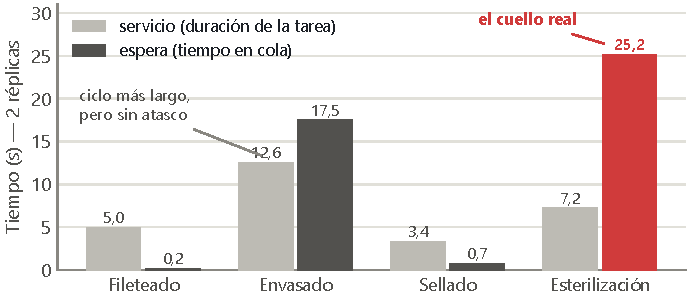
\includegraphics[width=0.95\linewidth]{fig_espera_vs_servicio.pdf}
\end{center}
\end{columns}
\end{frame}

% ── 11 · EL DETECTOR EN FUNCIONAMIENTO ───────────────────────────────────────
\begin{frame}
\titulo{El detector en funcionamiento}{La lógica que corre cada vez que alguien consulta el diagnóstico — y cómo la usamos para evidenciar el cuello}
\begin{columns}[T]
\column{0.50\textwidth}
\begin{itemize}
  \item \textbf{La regla}: \emph{advertencia} si la espera promedio (ventana de 60 s) supera $1{,}5\times$ el ciclo de la etapa; \emph{crítico} si supera $3\times$. El cuello es la etapa de \textbf{mayor espera} entre las que superan umbral; si ninguna, no hay cuello.
  \item \textbf{Cómo lo evidenciamos}: con la línea a ritmo constante, el detector señaló \textbf{envasado} (67,8 s). Agregamos una segunda envasadora: la espera bajó, pero la fila reapareció en \textbf{esterilización}. Con una tercera, envasado quedó sobrado — y el límite siguió ahí.
\end{itemize}
\column{0.46\textwidth}
\begin{center}
\begin{tikzpicture}
  \node (f1) [paso, minimum width=5.0cm] at (0,3.3) {las estaciones registran cada evento\\ (entra a cola · inicia · termina) en SQLite};
  \node (f2) [paso, minimum width=5.0cm] at (0,2.4) {la API de métricas promedia la espera\\ por etapa sobre los últimos 60 s};
  \node (f3) [paso, minimum width=5.0cm] at (0,1.6) {¿alguna espera $\geq 1{,}5\times$ su ciclo?};
  \node (f4a) [pasoc, minimum width=2.3cm] at (-1.45,0.55) {sin cuello:\\ línea normal};
  \node (f4b) [pasor, minimum width=2.5cm] at (1.45,0.55) {cuello = etapa de\\ mayor espera\\ ($\geq 3\times$: crítico)};
  \draw [arrow] (f1) -- (f2); \draw [arrow] (f2) -- (f3);
  \draw [arrow] (f3.south west) -- (f4a.north) node[font=\tiny, midway, left=2pt] {no};
  \draw [arrow] (f3.south east) -- (f4b.north) node[font=\tiny, midway, right=2pt] {sí};
\end{tikzpicture}
\end{center}
\end{columns}
\end{frame}

% ── 12 · DEMO ────────────────────────────────────────────────────────────────
\begin{frame}
\titulo{Demo en vivo}{El sistema completo, corriendo — tablero en \texttt{localhost:8501}}
\vspace{0.2cm}
\begin{columns}[T]
\column{0.55\textwidth}
{\small
\begin{enumerate}
  \item Línea al día: 4 etapas, 5 réplicas visibles con su ciclo y su carga.
  \item Ingresamos lotes desde la interfaz, espaciados ($\sim$5 s).
  \item La espera de esterilización crece en el gráfico: cartel \textcolor{ambar}{\textbf{ámbar}} $\to$ \textcolor{rojo}{\textbf{rojo}}, con la razón del diagnóstico.
  \item \textbf{Condición de carrera en vivo}: un botón corre lado a lado las dos versiones del reclamo con 100 órdenes. La versión en dos pasos registra $\sim$300 envasados para 100 órdenes (duplicados); la atómica, exactamente 100.
  \item Detenemos Redis: la interfaz \textbf{nombra al servicio caído} y el resto sigue vivo. Lo levantamos y todo continúa.
\end{enumerate}}
\column{0.41\textwidth}
\begin{beamercolorbox}[sep=8pt, rounded=true]{tarjetabox}
{\small\bfseries\color{marino}Qué mirar durante la demo}\\[3pt]
{\footnotesize\color{grisazul}El color marca \emph{importancia}, no identidad: lo normal es gris; el color fuerte queda reservado para advertencia y crítico, siempre con icono y texto.}
\end{beamercolorbox}
\vspace{0.25cm}
\cifra{1 comando}{\texttt{docker compose up} — despliegue completo}
\end{columns}
\end{frame}

% ── 13 · EXPERIMENTOS: PROTOCOLO ─────────────────────────────────────────────
\begin{frame}
\titulo{Experimentos: qué corrimos y por qué}{El mismo escenario, repetido con 1, 2 y 3 envasadoras — la corrida con 1 es la línea sin nuestro desarrollo}
\begin{center}
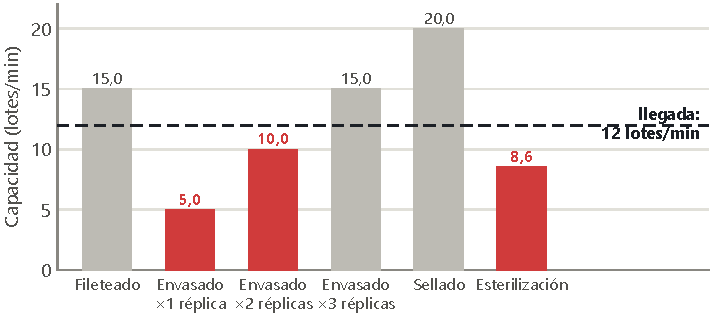
\includegraphics[width=0.50\linewidth]{fig_capacidad.pdf}
\end{center}
\begin{itemize}
  \item El experimento es software: un script crea \textbf{1 orden cada 5 s durante 180 s} vía la API de órdenes y al final consulta las métricas. Ritmo constante = demanda sostenida; inyectar de golpe mide otra cosa (prueba de saturación, aparte).
  \item La figura anticipa el resultado: toda etapa \textbf{bajo la línea de llegada} (12 lotes/min) acumulará fila. Con 2 réplicas, envasado sube a 10 — aún insuficiente — y esterilización (8,6) queda como siguiente límite.
\end{itemize}
\end{frame}

% ── 14 · RESULTADO CENTRAL ───────────────────────────────────────────────────
\begin{frame}
\titulo{El resultado central}{El cuello no se elimina al escalar: se muda de etapa}
\begin{center}
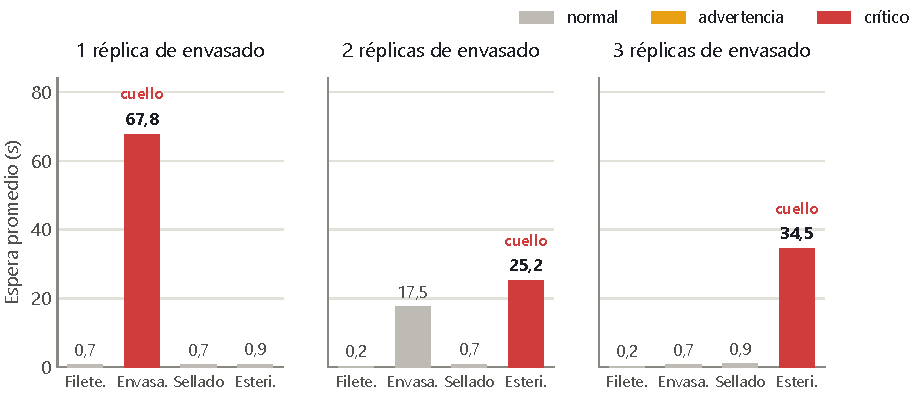
\includegraphics[width=0.70\linewidth]{fig_espera_replicas.pdf}
\end{center}
\begin{itemize}
  \item «Réplicas» = contenedores de envasado en paralelo sobre la misma cola: el equivalente a instalar 1, 2 o 3 \textbf{máquinas envasadoras}.
  \item Con 1 (la línea sin escalar), envasado acumula \textbf{67,8 s} de espera. Con 2, el cuello \textbf{se desplaza a esterilización}. Con 3, envasado queda sobrado (0,7 s)\dots{} y el cuello sigue en esterilización.
\end{itemize}
\end{frame}

% ── 15 · LEAD TIME ───────────────────────────────────────────────────────────
\begin{frame}
\titulo{¿Cuánto compra cada réplica?}{Lead time: lo que tarda una orden desde que se crea hasta que sale terminada}
\begin{center}
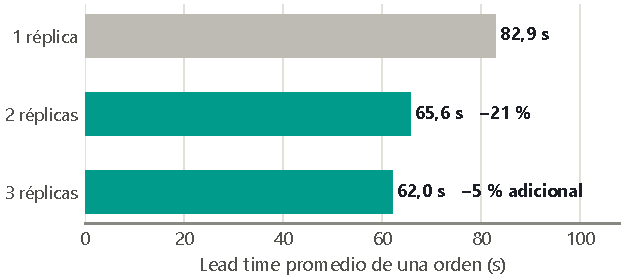
\includegraphics[width=0.6\linewidth]{fig_leadtime.pdf}
\end{center}
\begin{itemize}
  \item Frente a la línea sin escalar, la segunda envasadora reduce el lead time un \textbf{21 \%}; la tercera, casi nada: el límite ya no está en envasado.
  \item La siguiente inversión correcta sería \textbf{una segunda autoclave de esterilización}, no una tercera envasadora — y el tablero responde esa pregunta en vivo.
\end{itemize}
\end{frame}

% ── 16 · RÉPLICA LENTA ───────────────────────────────────────────────────────
\begin{frame}
\titulo{Balanceo con una réplica lenta}{Dos réplicas normales + una al doble de ciclo, sobre la misma cola, 30 lotes}
\begin{columns}[T]
\column{0.52\textwidth}
\begin{center}
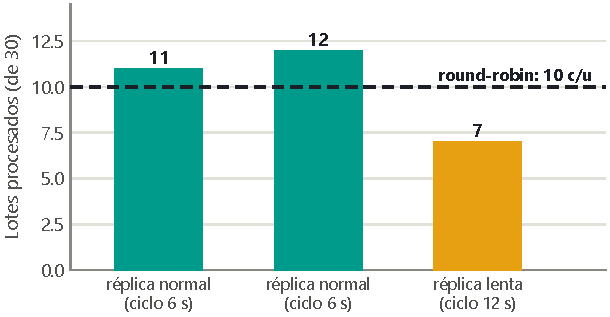
\includegraphics[width=\linewidth]{fig_replica_lenta.pdf}
\end{center}
\column{0.44\textwidth}
\vspace{0.4cm}
\begin{itemize}
  \item Un reparto por turnos (round-robin) habría dado \textbf{10/10/10} sin importar la velocidad — y la fila habría crecido frente a la lenta.
  \item El reparto \textbf{11/12/7} no lo programó nadie: emergió de que cada réplica pide trabajo solo al quedar libre.
  \item Eso es balanceo \emph{dinámico}: proporcional a la capacidad real de cada una, verificado con datos.
\end{itemize}
\end{columns}
\end{frame}

% ── 17 · SATURACIÓN ──────────────────────────────────────────────────────────
\begin{frame}
\titulo{Prueba de estrés: saturación}{Metimos 25 órdenes de golpe para verificar que el sistema detecta la congestión y se recupera sin operador}
\begin{columns}[T]
\column{0.56\textwidth}
\begin{center}
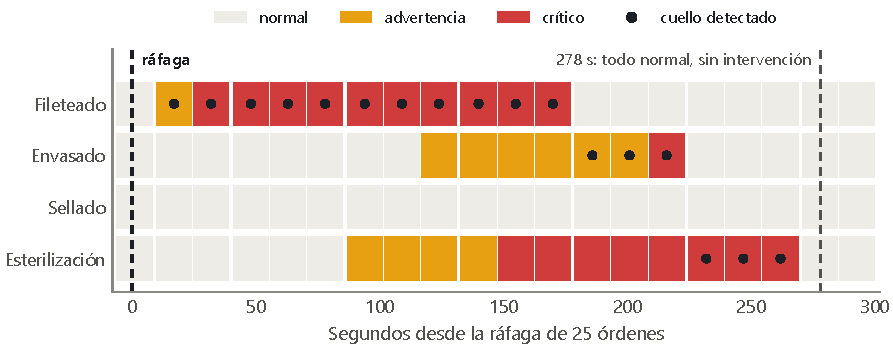
\includegraphics[width=0.94\linewidth]{fig_saturacion.pdf}
\end{center}
\begin{beamercolorbox}[sep=5pt, rounded=true]{tarjetabox}
{\footnotesize\color{grisazul}\textbf{Cómo leerlo:} cada fila es una etapa; cada celda, una consulta al diagnóstico (cada 15 s); el color, el estado que respondió.}
\end{beamercolorbox}
\column{0.40\textwidth}
\cifra{32 s}{el sistema declara \textbf{crítico} por sí solo, sin operador}
\cifra{278 s}{todo de vuelta en \textbf{normal}, sin intervención}
{\footnotesize\color{grisazul}\textbf{Qué nos dice:} el diagnóstico declara la congestión cuando aparece y la da de baja cuando pasa — la ventana móvil de 60 s deja ir las esperas viejas.}
\end{columns}
\end{frame}

% ── 18 · ERRORES ─────────────────────────────────────────────────────────────
\begin{frame}
\titulo{Qué pasa cuando una pieza se cae}{Provocamos la falla más grave —detener Redis, el reparto del trabajo— la medimos y la resolvimos}
\begin{columns}[T]
\column{0.48\textwidth}
\cifra{46 s}{\textbf{antes}: la API quedaba muda, sin error ni respuesta}
\column{0.48\textwidth}
\cifra{2,1 s}{\textbf{después}: respuesta inmediata que nombra al servicio caído}
\end{columns}
\vspace{0.3cm}
\begin{center}
\begin{tikzpicture}
  \node (e1) [paso, minimum width=3.7cm, minimum height=1.5cm] at (0,0) {\textbf{1 · Provocamos la falla}\\[2pt] detuvimos Redis con el\\ sistema corriendo};
  \node (e2) [paso, minimum width=4.5cm, minimum height=1.5cm] at (4.75,0) {\textbf{2 · Diagnosticamos}\\[2pt] el cuelgue no era la conexión:\\ era la resolución del nombre (DNS),\\ que el timeout no cubría};
  \node (e3) [pasoc, minimum width=4.5cm, minimum height=1.5cm] at (9.7,0) {\textbf{3 · Resolvimos}\\[2pt] plazo máximo de 2 s: si no hay\\ respuesta, error inmediato que\\ nombra al servicio caído};
  \draw [arrow] (e1) -- (e2); \draw [arrow] (e2) -- (e3);
\end{tikzpicture}
\end{center}
\vspace{0.2cm}
{\footnotesize\color{grisazul}La interfaz nunca muestra un error críptico: consulta la salud de los servicios y nombra al que realmente falta. El resto de los códigos de error (validación, orden inexistente) también está verificado contra el sistema corriendo.}
\end{frame}

% ── 19 · PERSISTENCIA Y REPRODUCIBILIDAD ─────────────────────────────────────
\begin{frame}
\titulo{Persistencia de datos}{Todo lo que la línea hace queda registrado — y por qué eso necesita una base de datos y no un archivo}
\begin{columns}[T]
\column{0.52\textwidth}
\begin{itemize}
  \item Cada acción de la línea (\emph{entra a cola} · \emph{inicia} · \emph{termina}) es un \textbf{evento} en SQLite. Las métricas se calculan siempre desde los eventos: \textbf{nada se guarda dos veces}, así ningún dato contradice a otro.
  \item Los datos sobreviven a apagar y levantar el sistema (verificado).
\end{itemize}
\vspace{0.05cm}
\begin{beamercolorbox}[sep=5pt, rounded=true]{tarjetabox}
{\small\bfseries\color{marino}¿Por qué una base de datos y no un archivo?}\\[2pt]
{\footnotesize\color{grisazul}Hasta 6 contenedores escriben \textbf{a la vez}: SQLite ordena esas escrituras para que entren de a una sin pisarse, y permite consultarlas con filtros. Un archivo compartido perdería o mezclaría escrituras.}
\end{beamercolorbox}
\column{0.44\textwidth}
{\footnotesize\color{grisazul}\textbf{La prueba de reproducibilidad}: en un computador limpio, descargamos el proyecto y \textbf{un solo comando} levantó el sistema completo.}\\[4pt]
\cifra{8/8}{de los 8 programas del sistema, los 8 arrancaron y confirmaron estar operativos}
\end{columns}
\end{frame}

% ── 20 · LÍMITES CONOCIDOS ───────────────────────────────────────────────────
\begin{frame}
\titulo{Límites conocidos y su solución}{Sabemos qué componente fallaría primero y cuál es el camino estándar de cada uno — sin rediseñar el resto}
\begin{center}
{\footnotesize\setlength{\tabcolsep}{5pt}
\begin{tabular}{L{2.6cm} L{4.9cm} L{5.3cm}}
\toprule
\textbf{Componente} & \textbf{Qué pasa hoy si falla} & \textbf{Solución estándar} \\
\midrule
Redis (las colas) & el reparto de trabajo se detiene: las estaciones quedan esperando & una copia de respaldo con conmutación automática (Redis Sentinel) \\
Una estación a mitad de ciclo & el lote que tenía en la mano se pierde de la línea & apartar el lote a una cola «en proceso» y devolverlo si la réplica deja de dar señales de vida \\
SQLite & atiende bien un nodo; con más escritores llegaría a su límite & migrar a un motor con servidor (PostgreSQL) cambiando un solo módulo \\
API / tablero & el operador pierde la interfaz; la línea sigue produciendo & una segunda instancia detrás de un balanceador HTTP \\
\bottomrule
\end{tabular}}
\end{center}
\vspace{0.15cm}
{\small Conocer el punto débil de cada componente también es parte del diseño — y la división en nodos hace cada mejora \textbf{local}: se toca un componente sin rediseñar los demás.}
\end{frame}

% ── 21 · CONCLUSIONES ────────────────────────────────────────────────────────
\begin{frame}
\titulo{Conclusiones}{Todo lo afirmado está respaldado por mediciones reproducibles}
\begin{columns}[T]
\column{0.48\textwidth}
\tarjeta{El cuello no se elimina: se desplaza}{De envasado a esterilización al pasar de 1 a 2 envasadoras; la tercera ya casi no mejora nada.}
\vspace{0.12cm}
\tarjeta{Medir la espera permite localizarlo}{El cuello real tenía un ciclo más corto que envasado: por tiempo de proceso no se habría encontrado.}
\vspace{0.12cm}
\tarjeta{El balanceo por demanda se adapta solo}{Reparto 11/12/7 con una réplica al doble de ciclo, sin que nadie lo asignara.}
\column{0.48\textwidth}
\tarjeta{La carrera se elimina, no se administra}{Extracción atómica: 0 duplicados en 200 órdenes, contra los duplicados del reclamo en dos pasos.}
\vspace{0.12cm}
\tarjeta{Las fallas se explican, no se enmascaran}{Con Redis caído, la API pasó de 46 s de silencio a responder en 2,1 s nombrando al servicio ausente.}
\end{columns}
\end{frame}

% ── 22 · GRACIAS ─────────────────────────────────────────────────────────────
\begin{frame}[plain]
\vfill
\begin{center}
{\dinfont\fontsize{40}{46}\selectfont\color{marino}Gracias}\\[14pt]
{\Large\color{grisazul}¿Preguntas?}\\[24pt]
{\color{tealu}\rule{2.2cm}{2pt}}\\[14pt]
{\small\color{grisazul}\texttt{github.com/CesarOlivares/Estructura-de-computadores-entrega-3}}
\end{center}
\vfill
\end{frame}

\end{document}
